\section{Motivation}

Let's consider the developement of a web-based bulletin board application, where
users can write their messages on a board, or request to read the current
messages on it.
In order to make the application scalable and highly
available, developers should implement it as a distributed application, working
with replicated data items, that runs on top of an off-the-shelf
eventually consistent data store. In this fashion, client requests are
sent to geo-replicated servers, where local updates are made, and each
update is guaranteed to be eventually delivered to all servers. 
\begin{figure}[t]
    \begin{subfigure}[b]{0.48\textwidth}
        \centering
	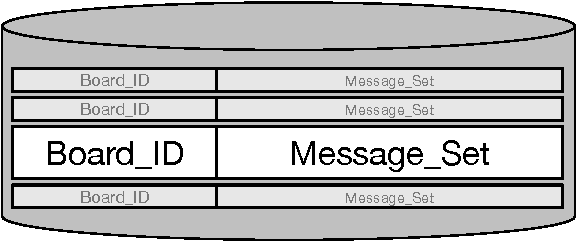
\includegraphics[scale = 0.5]{Figures/SimpleBulletinApp.pdf}
	\caption{Simple Data Model}
        \label{fig:simple_bb}
    \end{subfigure} 
    \begin{subfigure}[b]{0.48\textwidth}
        \centering
	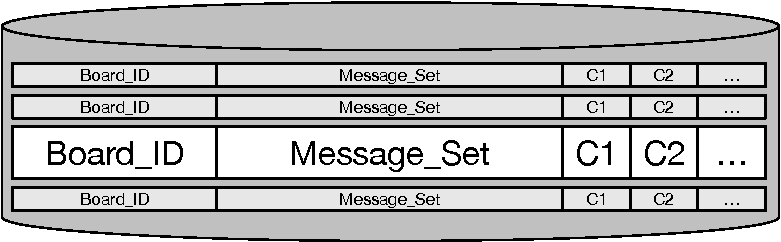
\includegraphics[scale=0.5]{Figures/ModifiedBulletinBoard.pdf}
	\caption{Modified Data Model}
	\label{fig:modified_bb}
    \end{subfigure}
    \\ \hrulefill \\
\caption{Low-Level Data Model of a Simple Bulletin Board Application
(Left) and the Modified Version Including Meta-data for Each Running
Session}
\label{fig:simple_modified_bb}
\end{figure}



\subsection{Ad-hoc Anomaly Prevention Mechanisms}
Developers cannot solely rely on the eventual consistency guarantee that
is provided by the stores. There are application integrity anomalies
that must be thought of at the developement stage and be fixed. For
example, assume the setting where Alice signs into the system, writes a
message on the board, and immediately refreshes her browser hoping to see
her message on the board, which is however not there. This is obviously
not desirable and as mentioned in
the previous section,  can occure if
the write message was sent to a server, and the subsequent read to
another, where the original update was not available yet. 

To prevent the above anomaly, developers must implement a consistency level known as 
Read My Writes (RMW), where users are guaranteed to see all their
previous updates whenever they read from a server. This would
obviously prevent the above anomaly, since Alice's read opertaion would
be blocked until her message arrives at the server. 





% Our approach
\subsection{Multi-Consistent Extension}
Doing these messy things is unavoidable, since the underlying stores,
only offer eventual consistency or if we are locky, one or two more
(such as causal consistency and strong consistency). But developers are
not interested in unnecessary consistency guaranteees and do it
themselves. There are so many of consistency known requirements and
there aren't generic ways of implementing them.
We are now arguing that all the consistency stuff can be
completely separated from the application level. We are proposing a
method that would completely liberate the developers from thinking about
these awful stuff. We are offering a shim that simply extends the
keyvalue store and preserves a consistency guarantee by recording
